\section{Further Development}
This section covers various features that could be implemented in future iterations of the system. Specifically

\subsection{Mobile Booking Application}
During early analysis, a mobile platform was suggested for implementation, but in the end the target platform chosen was the web. 
However, a simplified mobile application could be implemented, simplified in the sense that it would only provide login and booking functionality and not much else.
It would, however, also be an ideal platform for another further development feature, see \secref{subsec:closeststation}, given that GPS and internet connection are pervasive in modern mobile platforms.
The fact that you can take them with you makes them much more practical in the sense that you can determine at any time where the nearest station is.

\subsection{Closest Available Station}\label{subsec:closeststation}
During usability testing, one of the test subjects brought up an idea.
Specifically a feature that could be implemented on the website or as a mobile application is suggestion of closest available station.

The website could provide a suggestion of which station to go to based on distance where there is a bicycle free to use, where as the mobile application could suggest both the closest station with an available bicycle but also a station with an empty dock.
The closest station with an available bicycle can be used to see where the user would be able to get a bicycle, where as the available dock could be used when using a bicycle so you know where to go to deliver the bicycle to the station.

\subsection{Hotspot Detection}
In \chapref{sec:designAdminTools} a feature for administrators was suggested for showing 'hotspots' for bicycle activity. 
It was thought that it would allow administrators to more easily make decisions on where to place new stations, because if a hotspot showed areas with a lot of activity not close to any existing station, it would be logical to put a new station there.

However, questions about how the location data should be used were raised.
This meant more analysis on how to do it properly, and because of resource constraints this meant that no more development time would be dedicated to this feature. 
Specifically, should only location data where the bicycle has been at the same position for a long time be used? 
Should all location data be used, and would this not mean that popular routes would be hotspots as well and therefore be misleading? 

% Algorithms
There are many different ways of detecting hotspots, or clusters. One way is agglomerative clustering, others ways are K-Means, BIRCH, and DBSCAN.

Agglomerative would have worked by comparing the distances to all coordinates, which would have been very inefficient and thus not practical for a lot of points. 

K-Means could have worked but because it requires a specified amount K number of clusters, it is apparently not practical either. K-Means also includes outliers in existing clusters.

BIRCH and DBSCAN are made for large databases, which would likely be a benefit for this system given that a large amount of GPS coordinates would be registered, on the order of $10E5$ coordinates per bicycle per year. 

There are also simpler methods that might work, such as using a premade library for Google Maps API called MarkerClusterer that would greatly simplify the process but we do not know the algorithm it uses for clustering which could create performance problem. See \figref{fig:markerclusterer}.

\begin{figure}[h]
\begin{center}
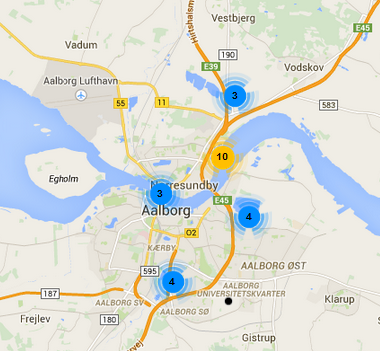
\includegraphics{MarkerClusterer}
\caption{The MarkerClusterer library produces this kind of result}
\label{fig:markerclusterer}
\end{center}
\end{figure}